\documentclass[]{article}
\usepackage{lmodern}
\usepackage{amssymb,amsmath}
\usepackage{ifxetex,ifluatex}
\usepackage{fixltx2e} % provides \textsubscript
\ifnum 0\ifxetex 1\fi\ifluatex 1\fi=0 % if pdftex
  \usepackage[T1]{fontenc}
  \usepackage[utf8]{inputenc}
\else % if luatex or xelatex
  \ifxetex
    \usepackage{mathspec}
  \else
    \usepackage{fontspec}
  \fi
  \defaultfontfeatures{Ligatures=TeX,Scale=MatchLowercase}
\fi
% use upquote if available, for straight quotes in verbatim environments
\IfFileExists{upquote.sty}{\usepackage{upquote}}{}
% use microtype if available
\IfFileExists{microtype.sty}{%
\usepackage[]{microtype}
\UseMicrotypeSet[protrusion]{basicmath} % disable protrusion for tt fonts
}{}
\PassOptionsToPackage{hyphens}{url} % url is loaded by hyperref
\usepackage[unicode=true]{hyperref}
\hypersetup{
            pdfborder={0 0 0},
            breaklinks=true}
\urlstyle{same}  % don't use monospace font for urls
\usepackage{graphicx,grffile}
\makeatletter
\def\maxwidth{\ifdim\Gin@nat@width>\linewidth\linewidth\else\Gin@nat@width\fi}
\def\maxheight{\ifdim\Gin@nat@height>\textheight\textheight\else\Gin@nat@height\fi}
\makeatother
% Scale images if necessary, so that they will not overflow the page
% margins by default, and it is still possible to overwrite the defaults
% using explicit options in \includegraphics[width, height, ...]{}
\setkeys{Gin}{width=\maxwidth,height=\maxheight,keepaspectratio}
\IfFileExists{parskip.sty}{%
\usepackage{parskip}
}{% else
\setlength{\parindent}{0pt}
\setlength{\parskip}{6pt plus 2pt minus 1pt}
}
\setlength{\emergencystretch}{3em}  % prevent overfull lines
\providecommand{\tightlist}{%
  \setlength{\itemsep}{0pt}\setlength{\parskip}{0pt}}
\setcounter{secnumdepth}{0}
% Redefines (sub)paragraphs to behave more like sections
\ifx\paragraph\undefined\else
\let\oldparagraph\paragraph
\renewcommand{\paragraph}[1]{\oldparagraph{#1}\mbox{}}
\fi
\ifx\subparagraph\undefined\else
\let\oldsubparagraph\subparagraph
\renewcommand{\subparagraph}[1]{\oldsubparagraph{#1}\mbox{}}
\fi

% set default figure placement to htbp
\makeatletter
\def\fps@figure{htbp}
\makeatother


\date{}

\begin{document}

Zipeng Wang \#3909934

\section{Physics 129L HW8 Ex1 Report}\label{physics-129l-hw8-ex1-report}

Each background pdf has been normalized such that the area under the
curve from \(mass = 100(GeV)\) to \(mass = 200(GeV)\) is 1.
Normalization constants are recorded in the code ``hw8\_ex1.py''.

\subsection{Fit 1: Exponential}\label{fit-1-exponential}

In this trial I used the background pdf \(e^{-\alpha x}\).

Result: Analyzed by Minos, the fitted value for S is
\(S = 22.6^{+ 8.12}_{-7.5}\). The fitted value for B is
\(B=177^{+15.1}_{-14.3}\).

In my opinion, this fit is not very reasonable because there is large
disagreement between \(mass = 180\) and \(mass = 200\). It seems that
the background is concave down instead of concave up.

\begin{figure}
\centering
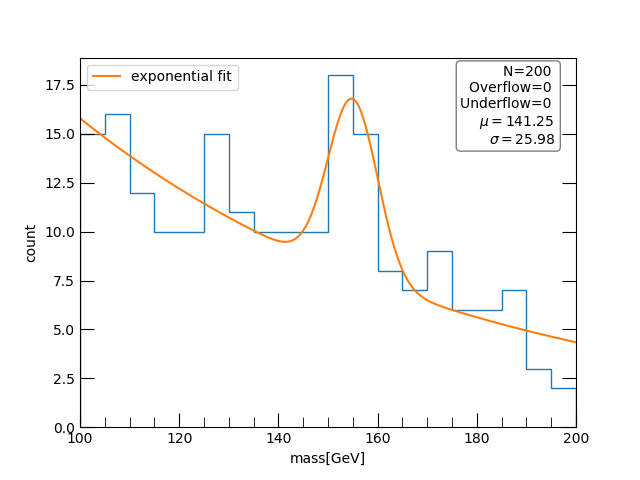
\includegraphics{./ex1_figs/Fit1_exponential.png}
\caption{Exponential Fit}
\end{figure}

\subsection{Fit 2: Linear}\label{fit-2-linear}

In this trial I used a linear background pdf \(-kx+b\).

Result: Analyzed by Minos, the fitted value for S is
\(S = 20.2^{+ 7.99}_{-7.39}\). The fitted value for B is
\(B=180^{+15.2}_{-14.4}\).

I think this is a good fit since there is no obvious deviation between
data and fit, though the underlying physics in this problem might not be
as simple as linear. However, based on the information at hand, I think
this is a good enough fit.

\begin{figure}
\centering
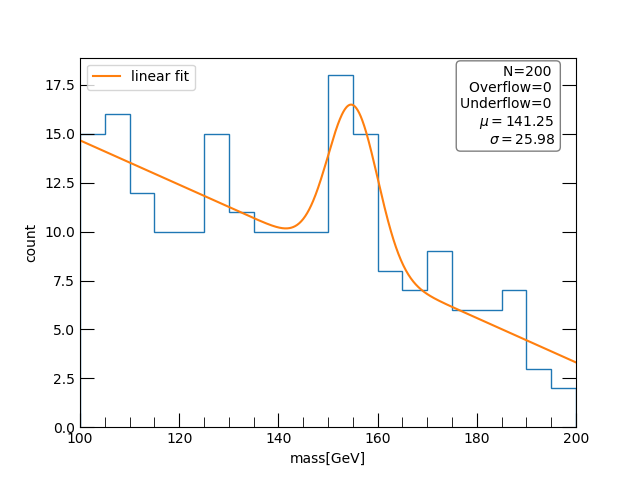
\includegraphics{./ex1_figs/Fit2_linear.png}
\caption{Linear Fit}
\end{figure}

\subsection{Fit 3: Quadratic}\label{fit-3-quadratic}

In this trial I used a quadratic polynomial background pdf
\(-ax^2 +bx+c\).

Result: Analyzed by Minos, the fitted value for S is
\(S = 18.6^{+ 8.81}_{-8.25}\). The fitted value for B is
\(B=181^{+15.8}_{-14.9}\).

I think this fit is the best among the three fits I tried. It is the
closest to the binned data. Also, any pdf with some curvature can be
approximated by a quadratic, so I think this fit shows some general
characteristics for all the concave down background pdfs.

\begin{figure}[h]
\centering
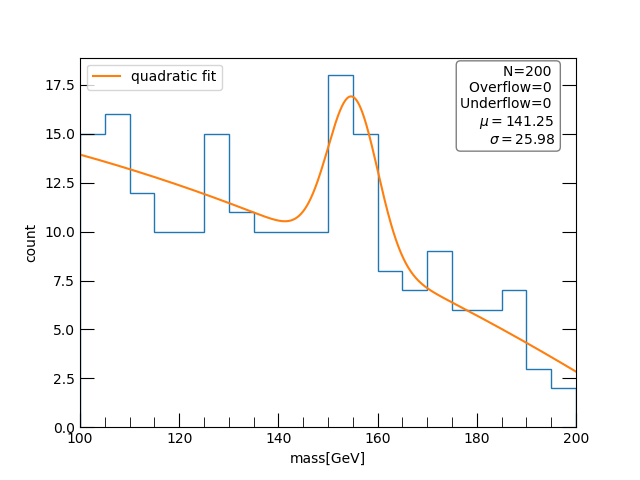
\includegraphics{./ex1_figs/Fit3_quadratic.png}
\caption{Quadratic Fit}
\end{figure}

\subsection{Final Result}\label{final-result}

Overall, these three different fits gives the value of S ranging from
\(18.6\) to \(22.6\). Therefore, I estimate that the systematic error
here is \(\pm 2\).

The value of S is \(S = 18.6 \pm 8.52 \pm 2\).

\end{document}
